\subsection{Interval Timers}
\label{sec:interval_port}

The {\it \systemNameFull} includes a timer module implemented in the FPGA that can be used by
the \processor~processor. This timer can be loaded with a preset value, and then counts down to 
zero using a 100-MHz clock. The programming interface 
for the timer includes six 16-bit registers, as illustrated in Figure~\ref{fig:interval_port}.  
The 16-bit register at address {\sf 0xFF202000} provides status information about the timer,
and the register at address {\sf 0xFF202004} allows control settings to be made.  The bit 
fields in these registers are described below:

\begin{itemize}
\item
{\it TO} provides a timeout signal which is set to 1 by the timer when it 
has reached a count value of zero.  The {\it TO} bit can be reset by writing a 0 into it. 
\item 
{\it RUN} is set to 1 by the timer whenever it is currently counting. Write 
operations to the status halfword do not affect the value of the {\it RUN} bit. 

\item 
{\it ITO} is used for generating interrupts, which are discussed in section \ref{sec:exceptions}.

\begin{figure}[h!]
   \begin{center}
       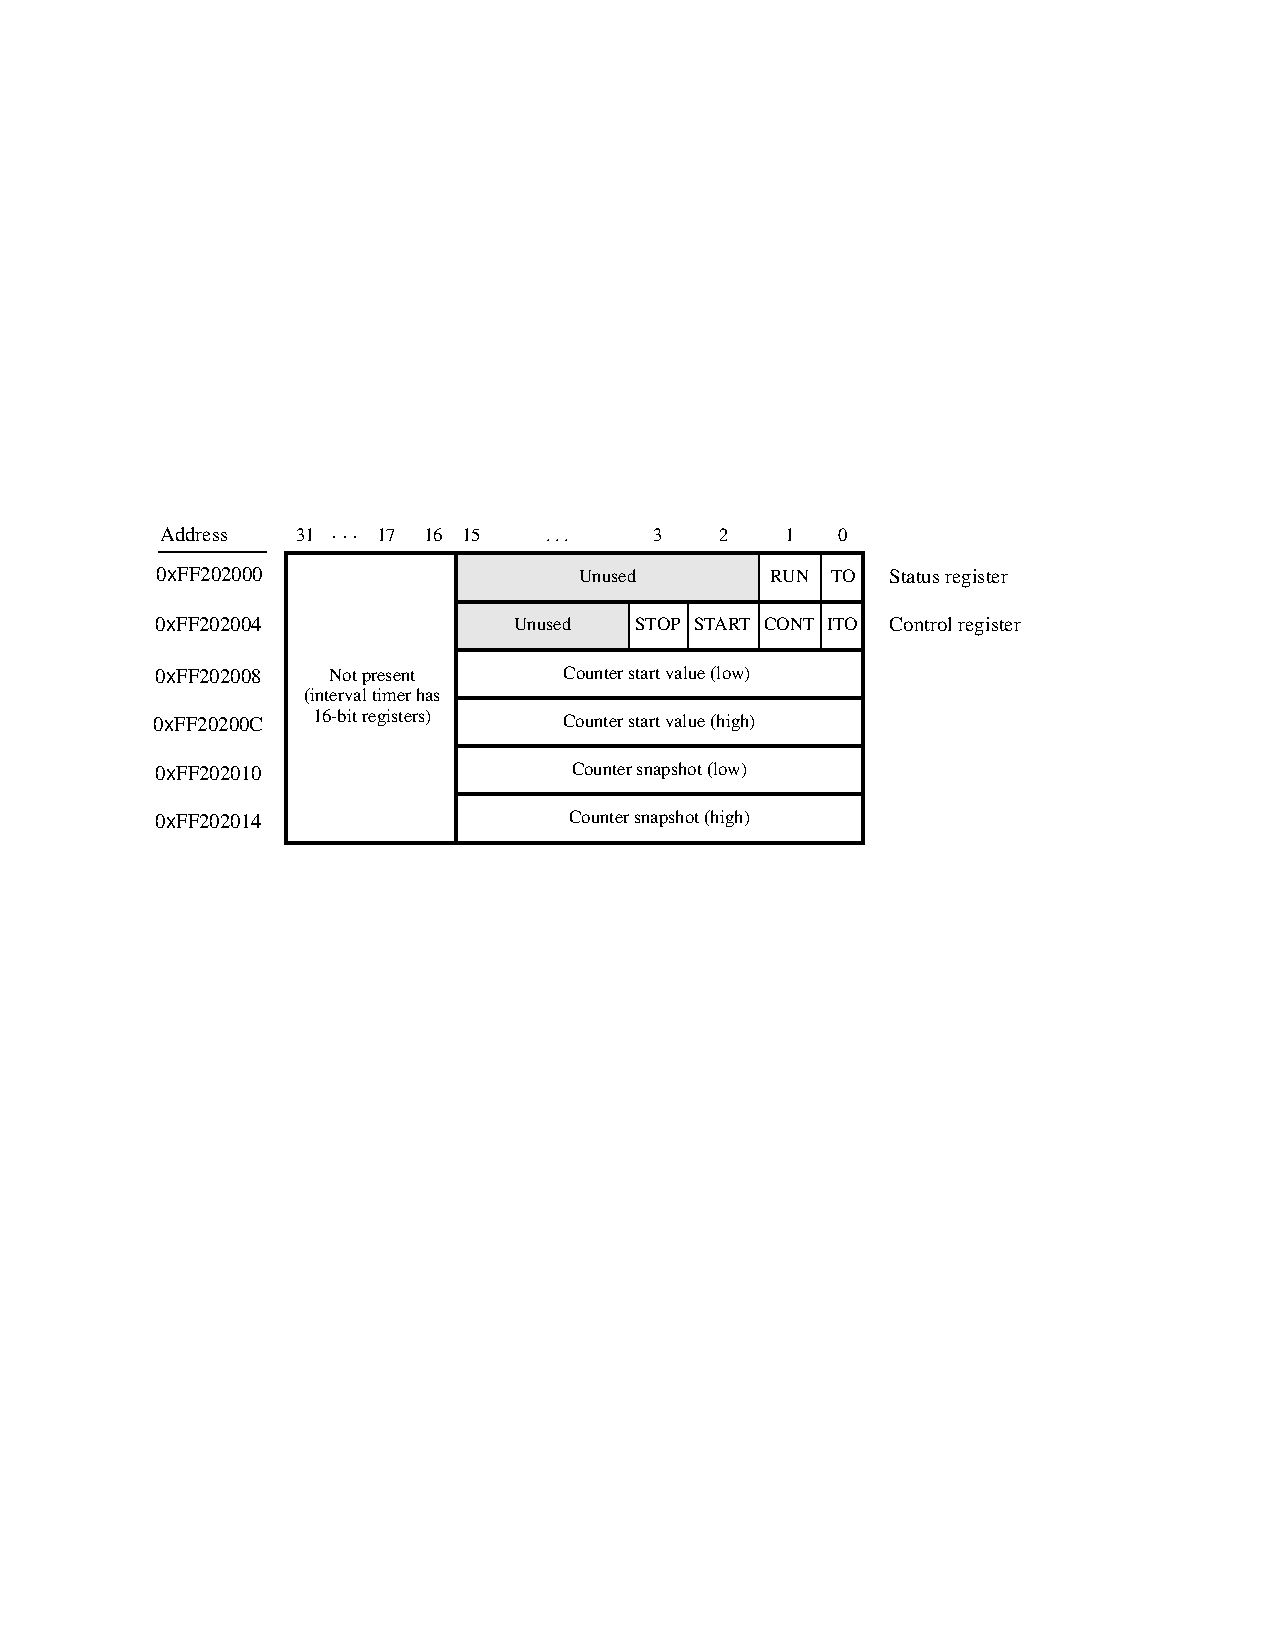
\includegraphics{../../../common/figs/FPGA_Interval_Timers.pdf}
   \end{center}
   \caption{Interval timer registers.}
	\label{fig:interval_port}
\end{figure}

\item
{\it CONT} affects the continuous operation of the timer.  When the timer reaches
a count value of zero it automatically reloads the specified starting count value. If 
{\it CONT} is set to 1, then the timer will continue counting down automatically.
But if {\it CONT} $=0$, then the timer will stop after it has reached a count value of 0. 

\item
({\it START}/{\it STOP}) is used to commence/suspend the operation of the 
timer by writing a 1 into the respective bit.
\end{itemize}

The two 16-bit registers at addresses {\sf 0xFF202008} and {\sf 0xFF20200C}
allow the period of the timer to be changed by
setting the starting count value.  The default setting gives a timer period of 125 msec. 
To achieve this period, the starting value of the count is
100 MHz $\times$ 125 msec $=12.5\times10^6$. It is possible to capture a snapshot of the 
counter value at any time by performing a write to address {\sf 0xFF202010}. This write
operation causes the current 32-bit counter value to be stored into the two 16-bit timer
registers at addresses {\sf 0xFF202010} and {\sf 0xFF202014}. These registers can then be
read to obtain the count value.

A second interval timer, which has an identical interface to the one described above, is also 
available in the FPGA, starting at the base address {\sf 0xFF202020}.

